% !TEX root = trkjet.tex

\part*{Auxiliary material}
\addcontentsline{toc}{part}{Auxiliary material}
%-------------------------------------------------------------------------------

%In an ATLAS paper, auxiliary plots and tables that are supposed to be made public 
%should be collected in an appendix that has the title \enquote{Auxiliary material}.
%This information will appear on the public webpage, but will not be included
%in the document submitted to arXiv and to the journal.

%
%\begin{figure}[h]
%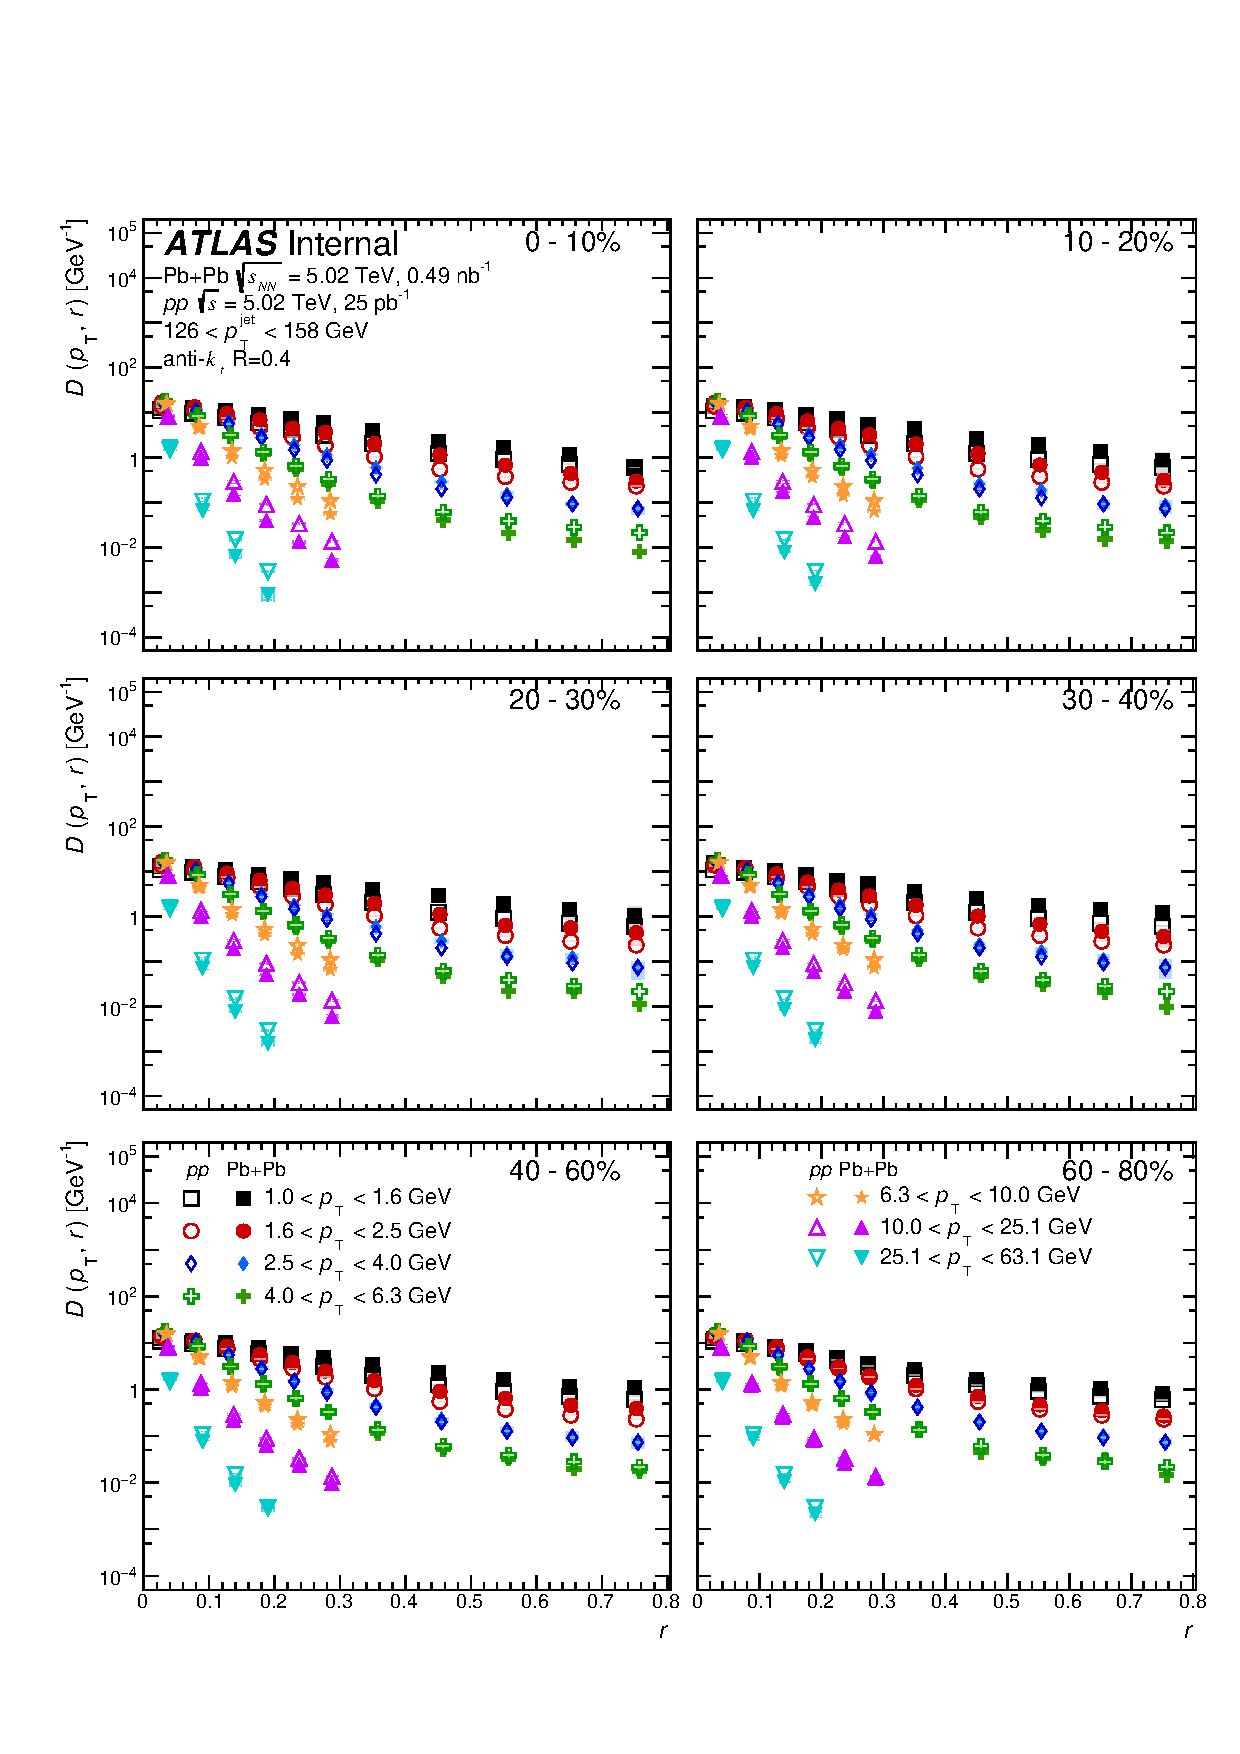
\includegraphics[width=1.0\textwidth]{figures/results/DpT_dR_jet7}
%\caption{ \Dptr\ distributions as a function of \rvar\ for different \pt\ ranges in 126--158 GeV jets. The open markers are for \pp\ collisions and the solid markers are for \pbpb\ collisions. The different panels refer to different centrality selections}
%\label{fig:fullset_dptr_j7}
%\end{figure}

\begin{figure}[h]
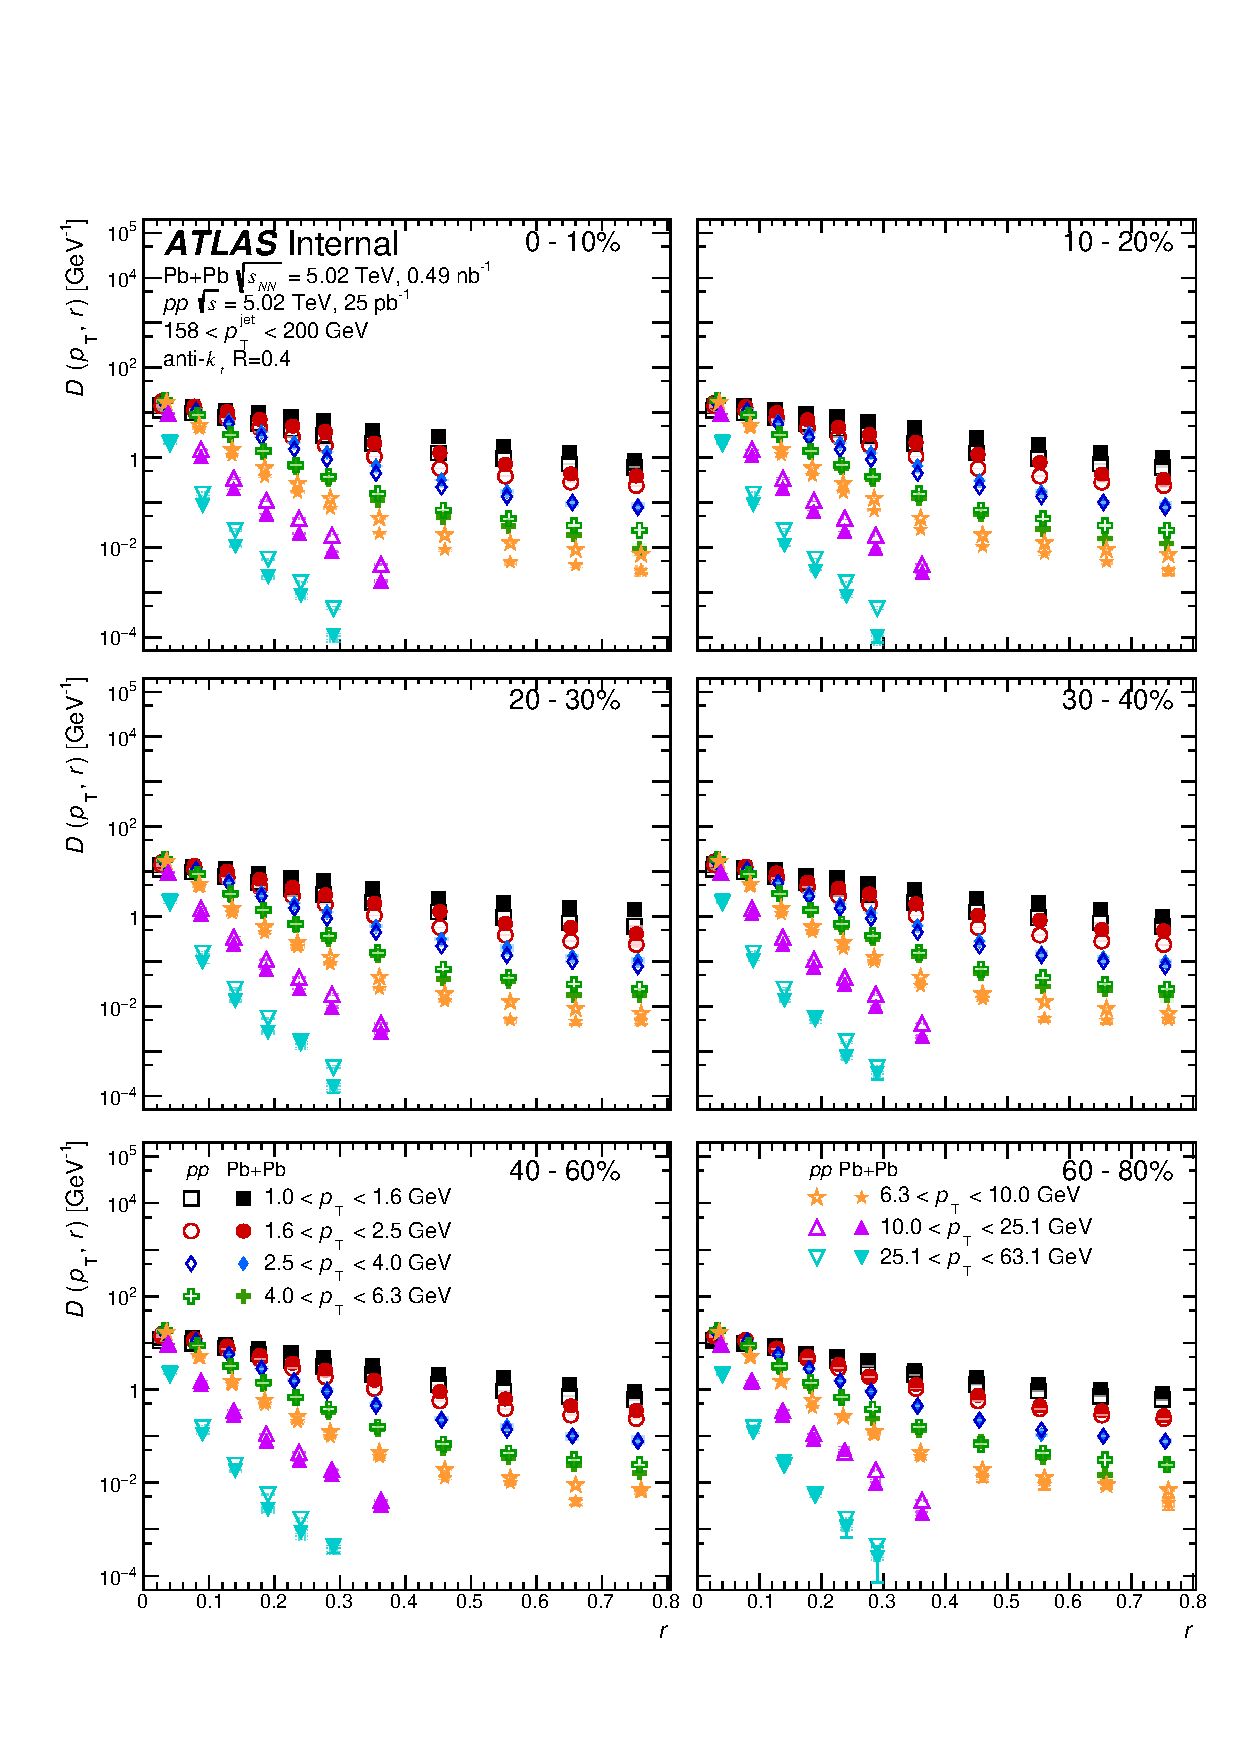
\includegraphics[width=1.0\textwidth]{figures/results/DpT_dR_jet8}
\caption{ \Dptr\ distributions as a function of \rvar\ for different \pt\ ranges in 158--200 GeV jets. The open markers are for \pp\ collisions and the solid markers are for \pbpb\ collisions. The different panels refer to different centrality selections}
\label{fig:fullset_dptr_j8}
\end{figure}

\begin{figure}[h]
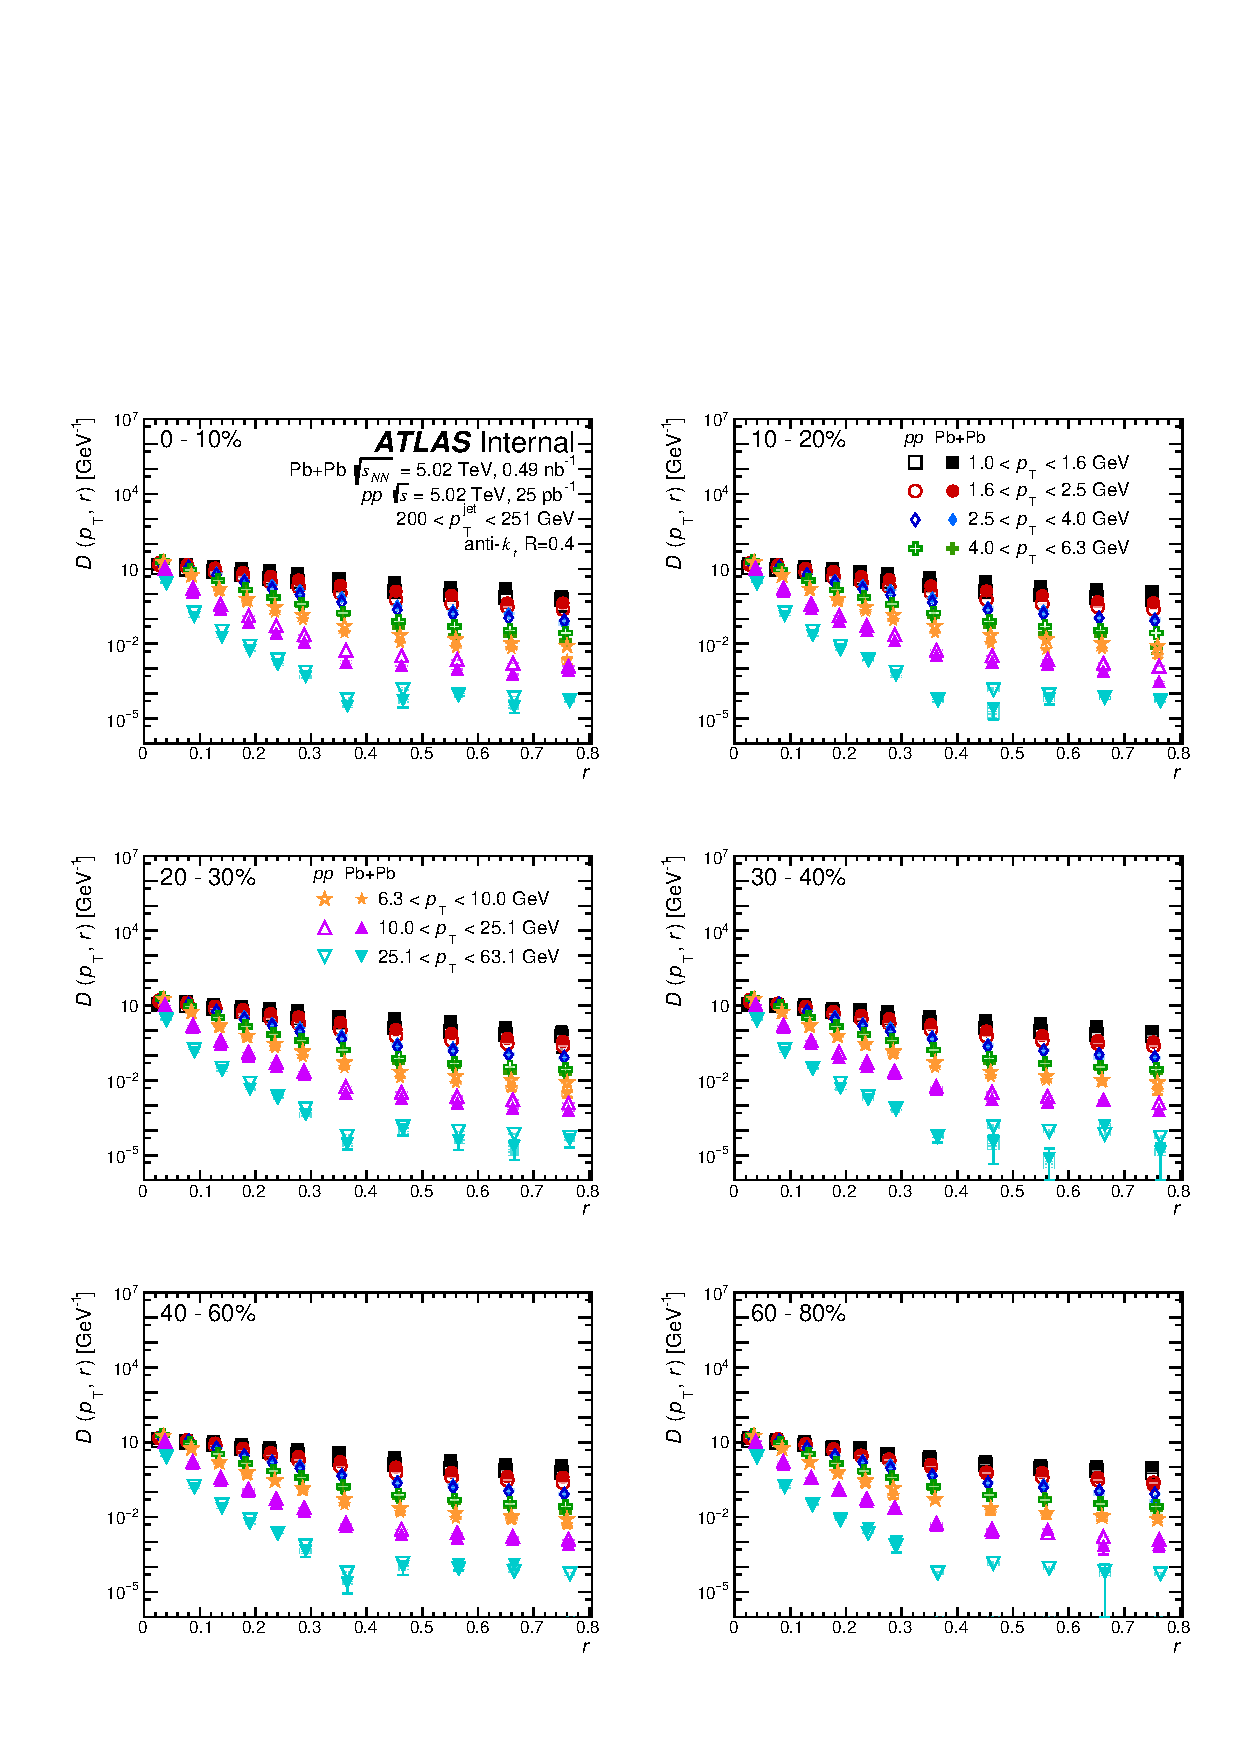
\includegraphics[width=1.0\textwidth]{figures/results/DpT_dR_jet9}
\caption{ \Dptr\ distributions as a function of \rvar\ for different \pt\ ranges in 200--251 GeV jets. The open markers are for \pp\ collisions and the solid markers are for \pbpb\ collisions. The different panels refer to different centrality selections}
\label{fig:fullset_dptr_j9}
\end{figure}

\begin{figure}[h]
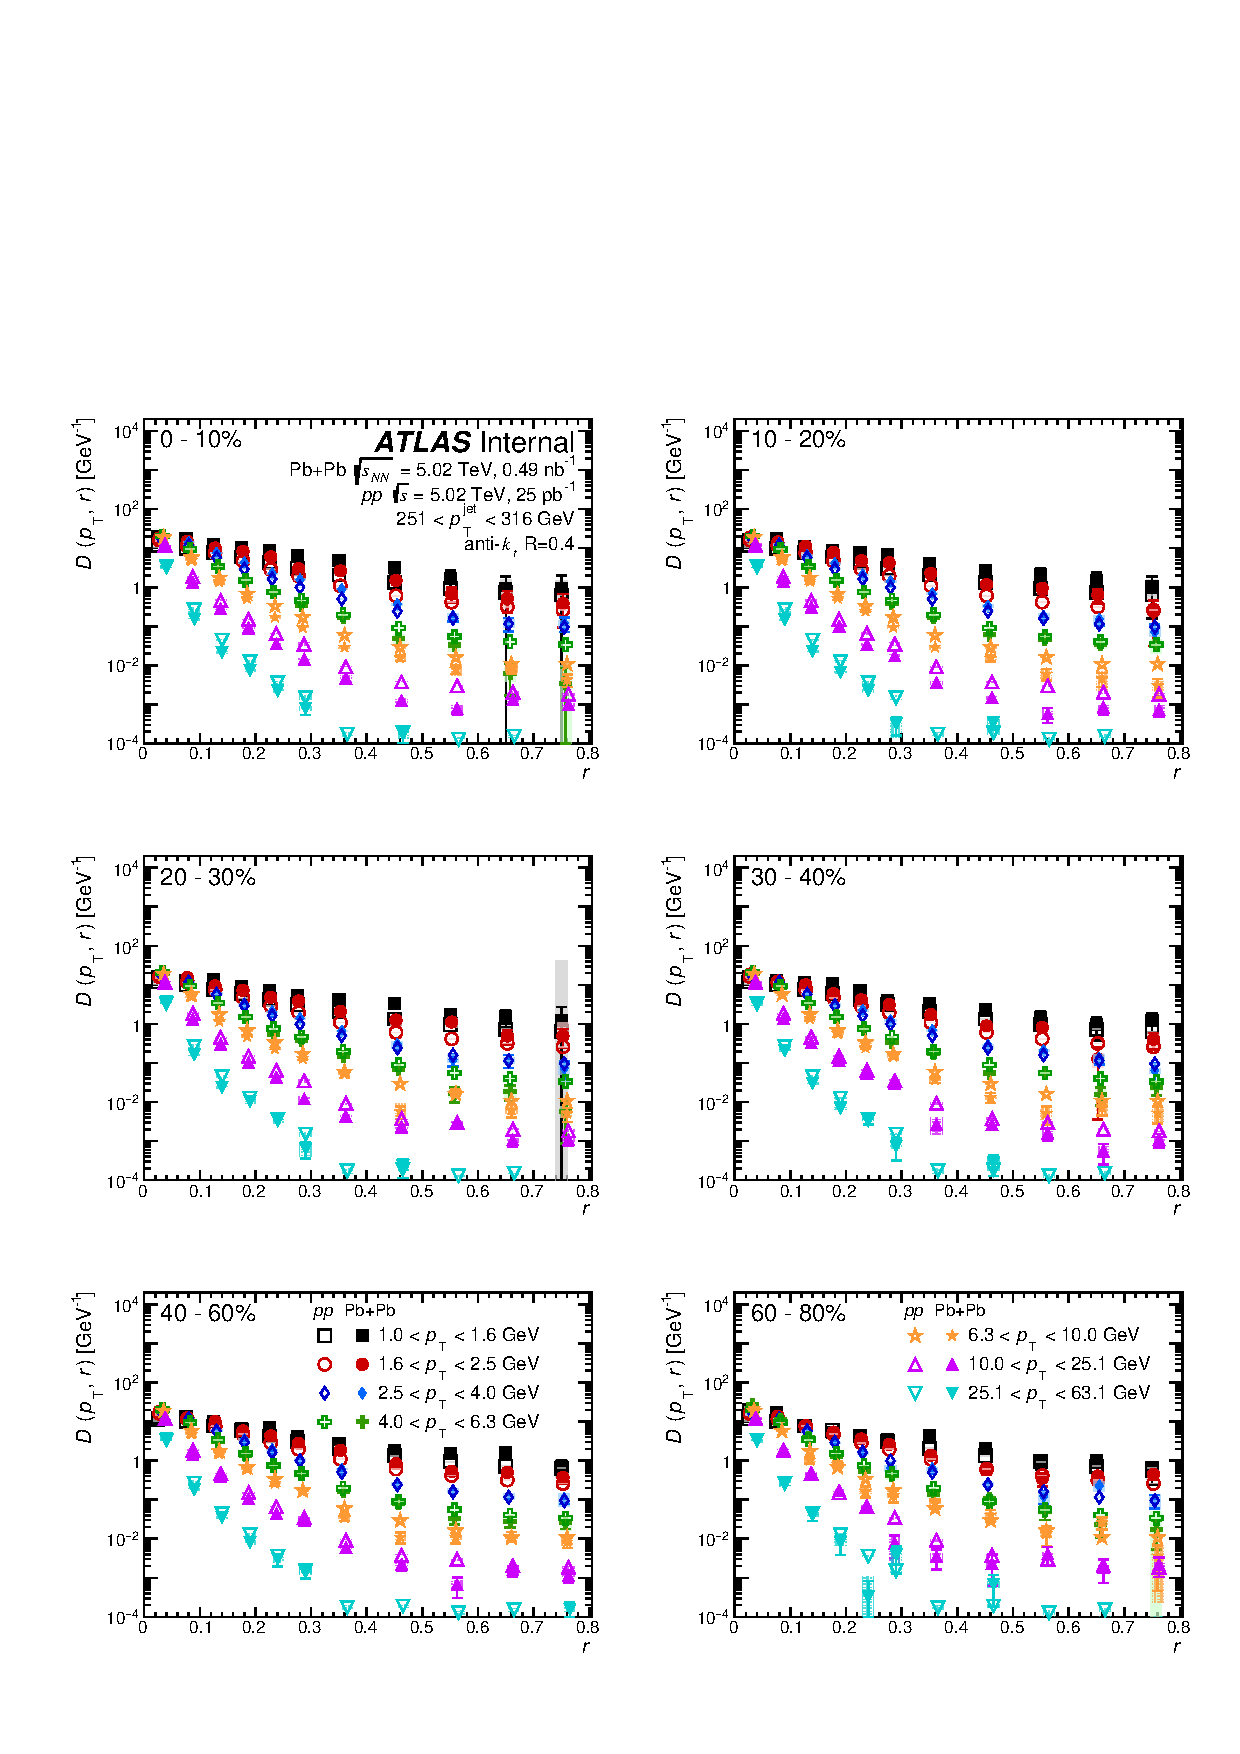
\includegraphics[width=1.0\textwidth]{figures/results/DpT_dR_jet10}
\caption{ \Dptr\ distributions as a function of \rvar\ for different \pt\ ranges in 251--316 GeV jets. The open markers are for \pp\ collisions and the solid markers are for \pbpb\ collisions. The different panels refer to different centrality selections}
\label{fig:fullset_dptr_j10}
\end{figure}


\begin{figure}[h]
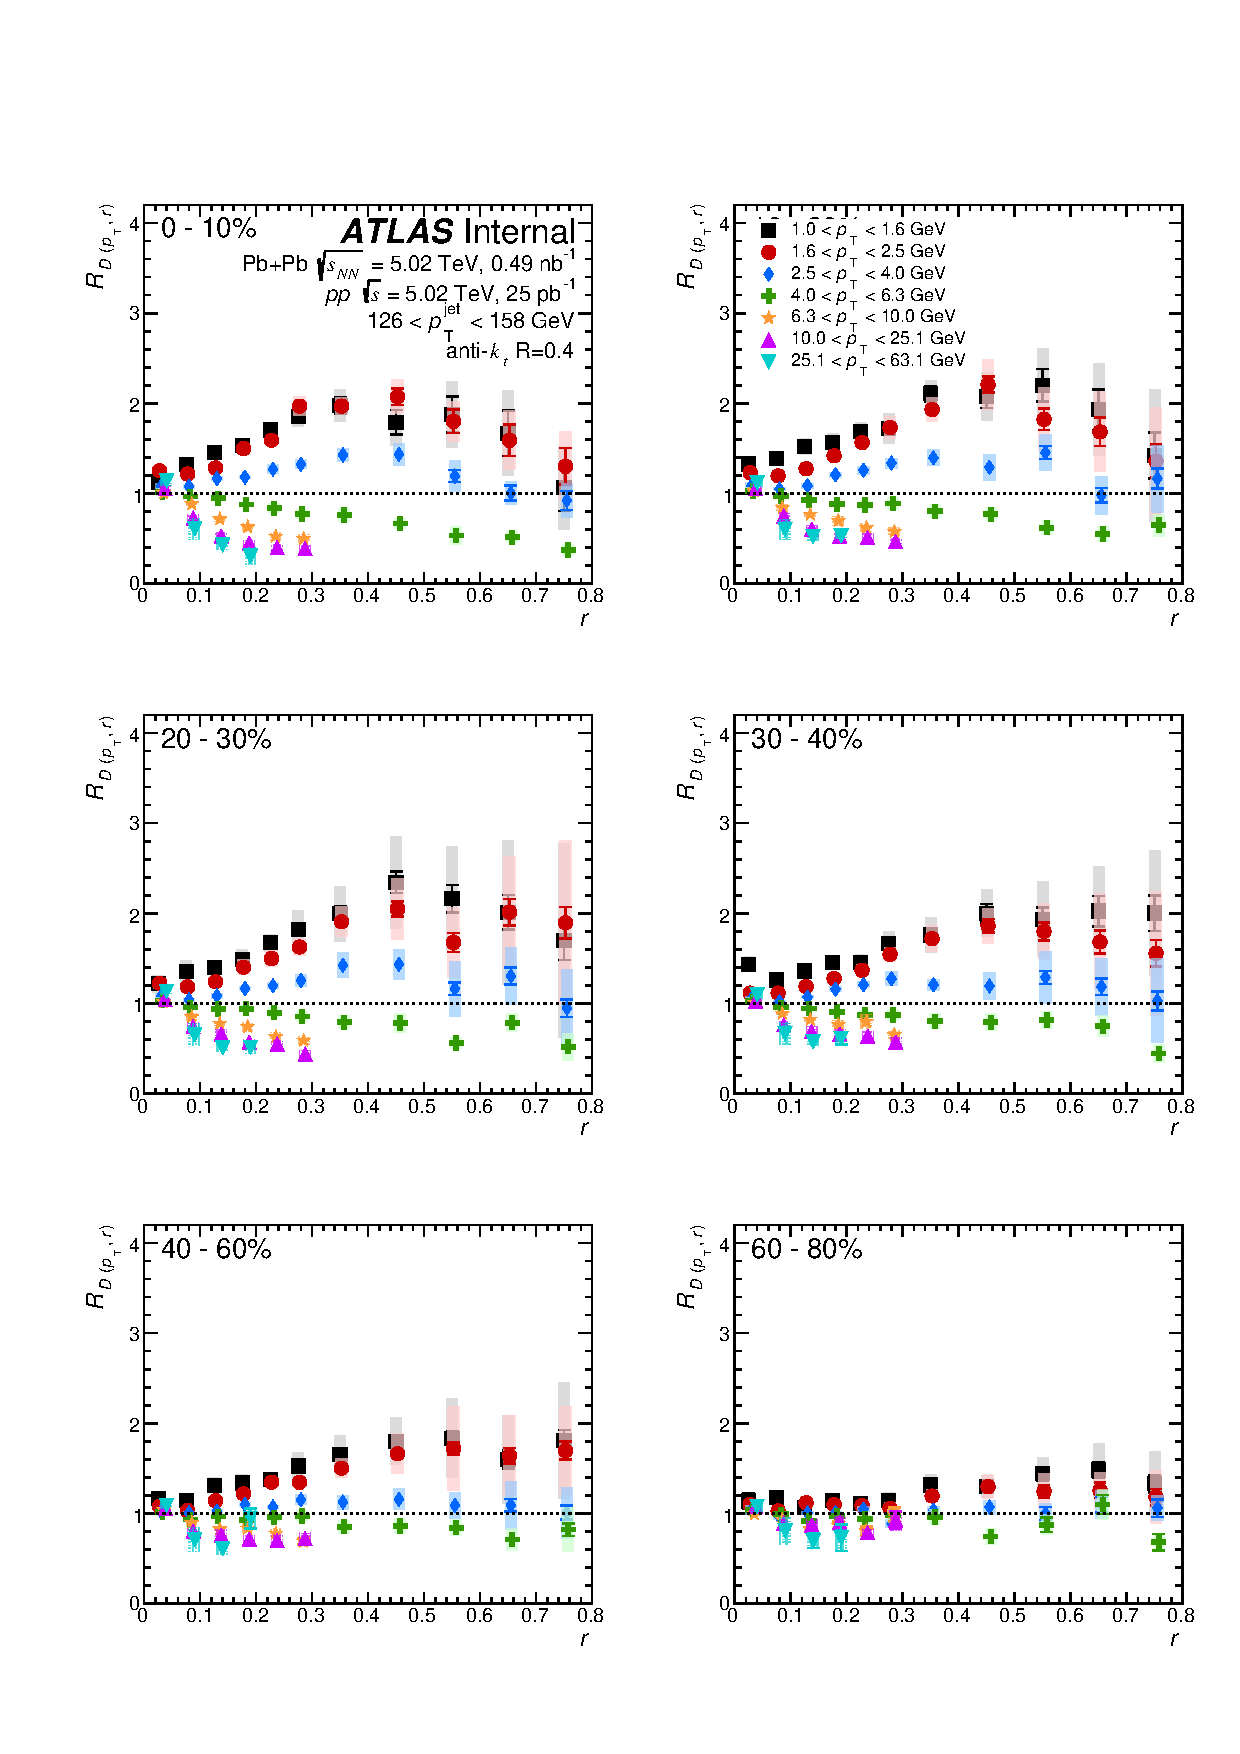
\includegraphics[width=1.0\textwidth]{figures/results/RDpT_dR_jet7}
\caption{The \RDptr\ distributions as a function of \rvar\ for different \pt\ selections in 126--158 GeV jets. The different panels refer to different centrality selections.}
\label{fig:fullset_rptr_j7}
\end{figure}

\begin{figure}[h]
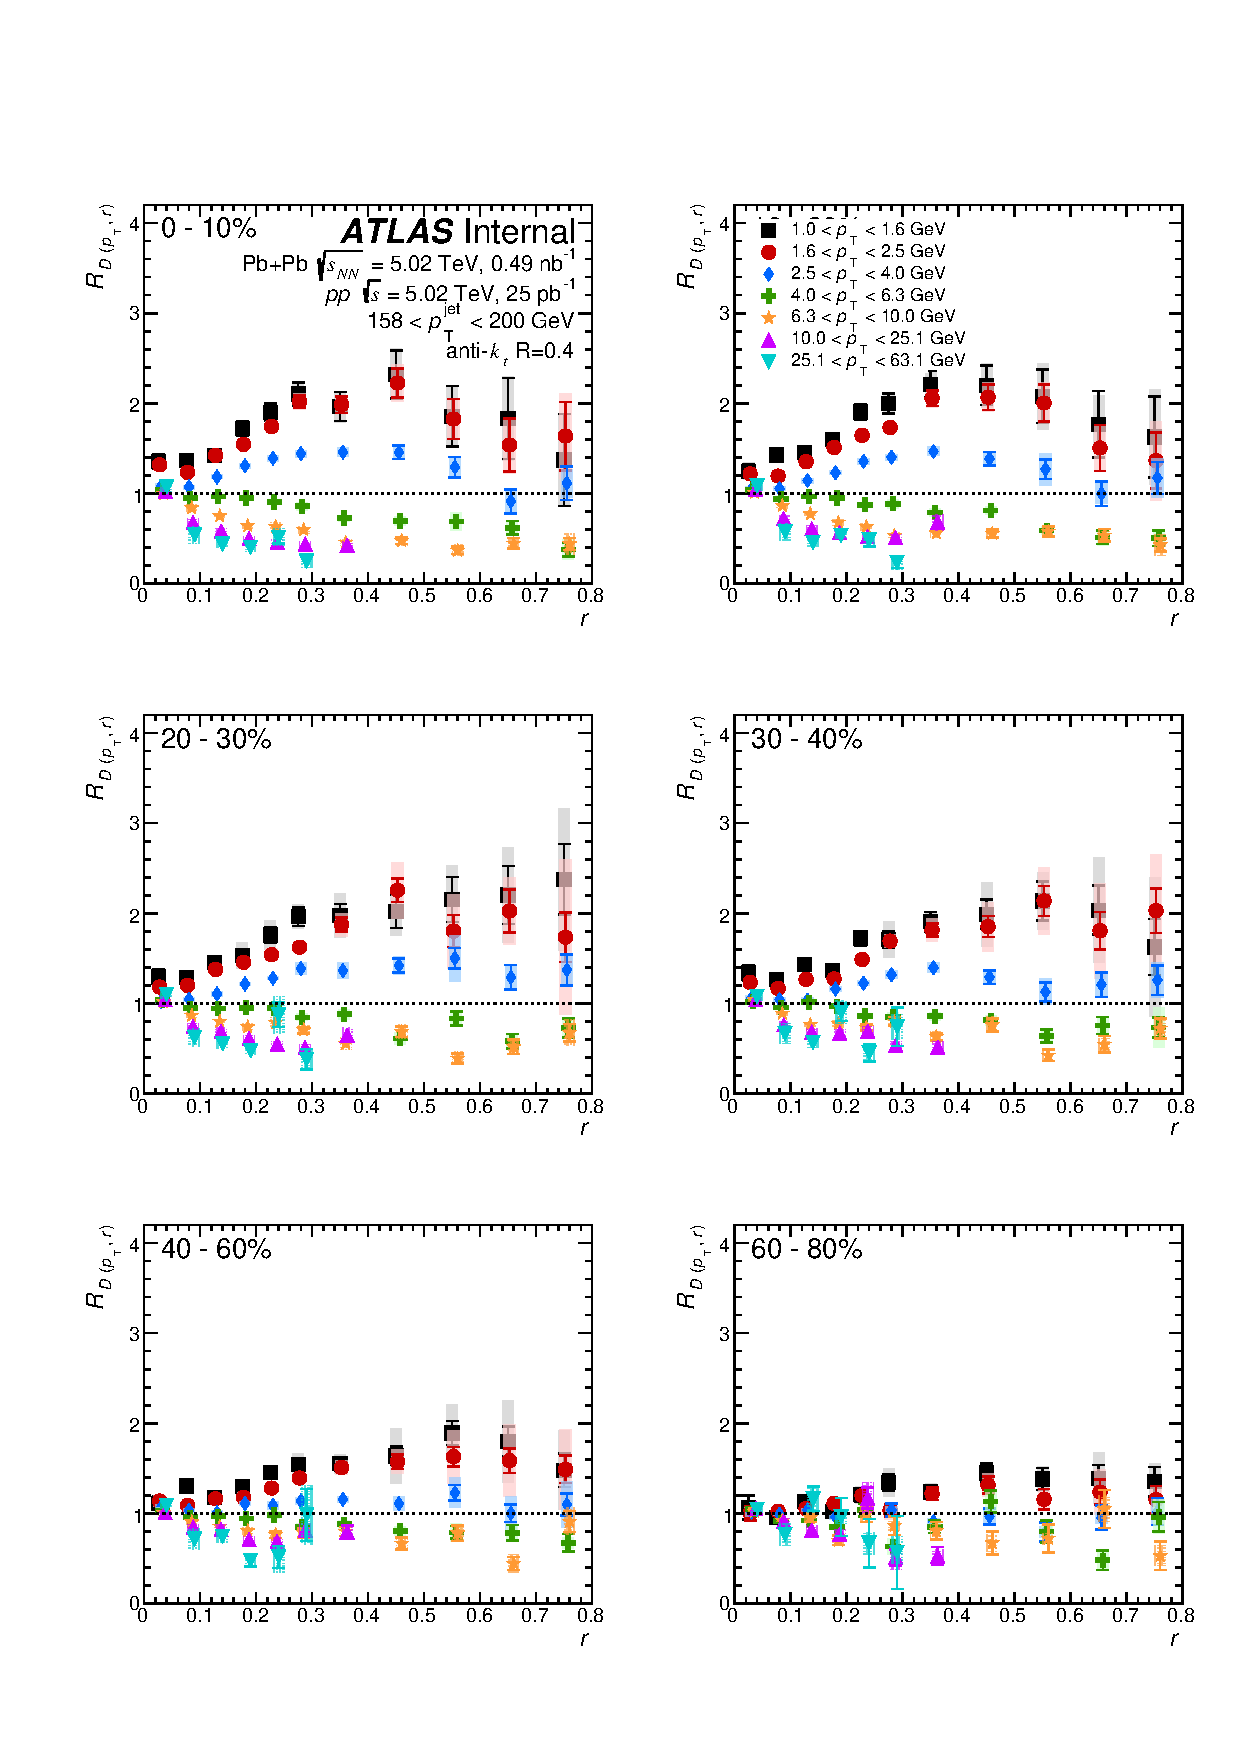
\includegraphics[width=1.0\textwidth]{figures/results/RDpT_dR_jet8}
\caption{The \RDptr\ distributions as a function of \rvar\ for different \pt\ selections in 158--200 GeV jets. The different panels refer to different centrality selections.}
\label{fig:fullset_rptr_j8}
\end{figure}

\begin{figure}[h]
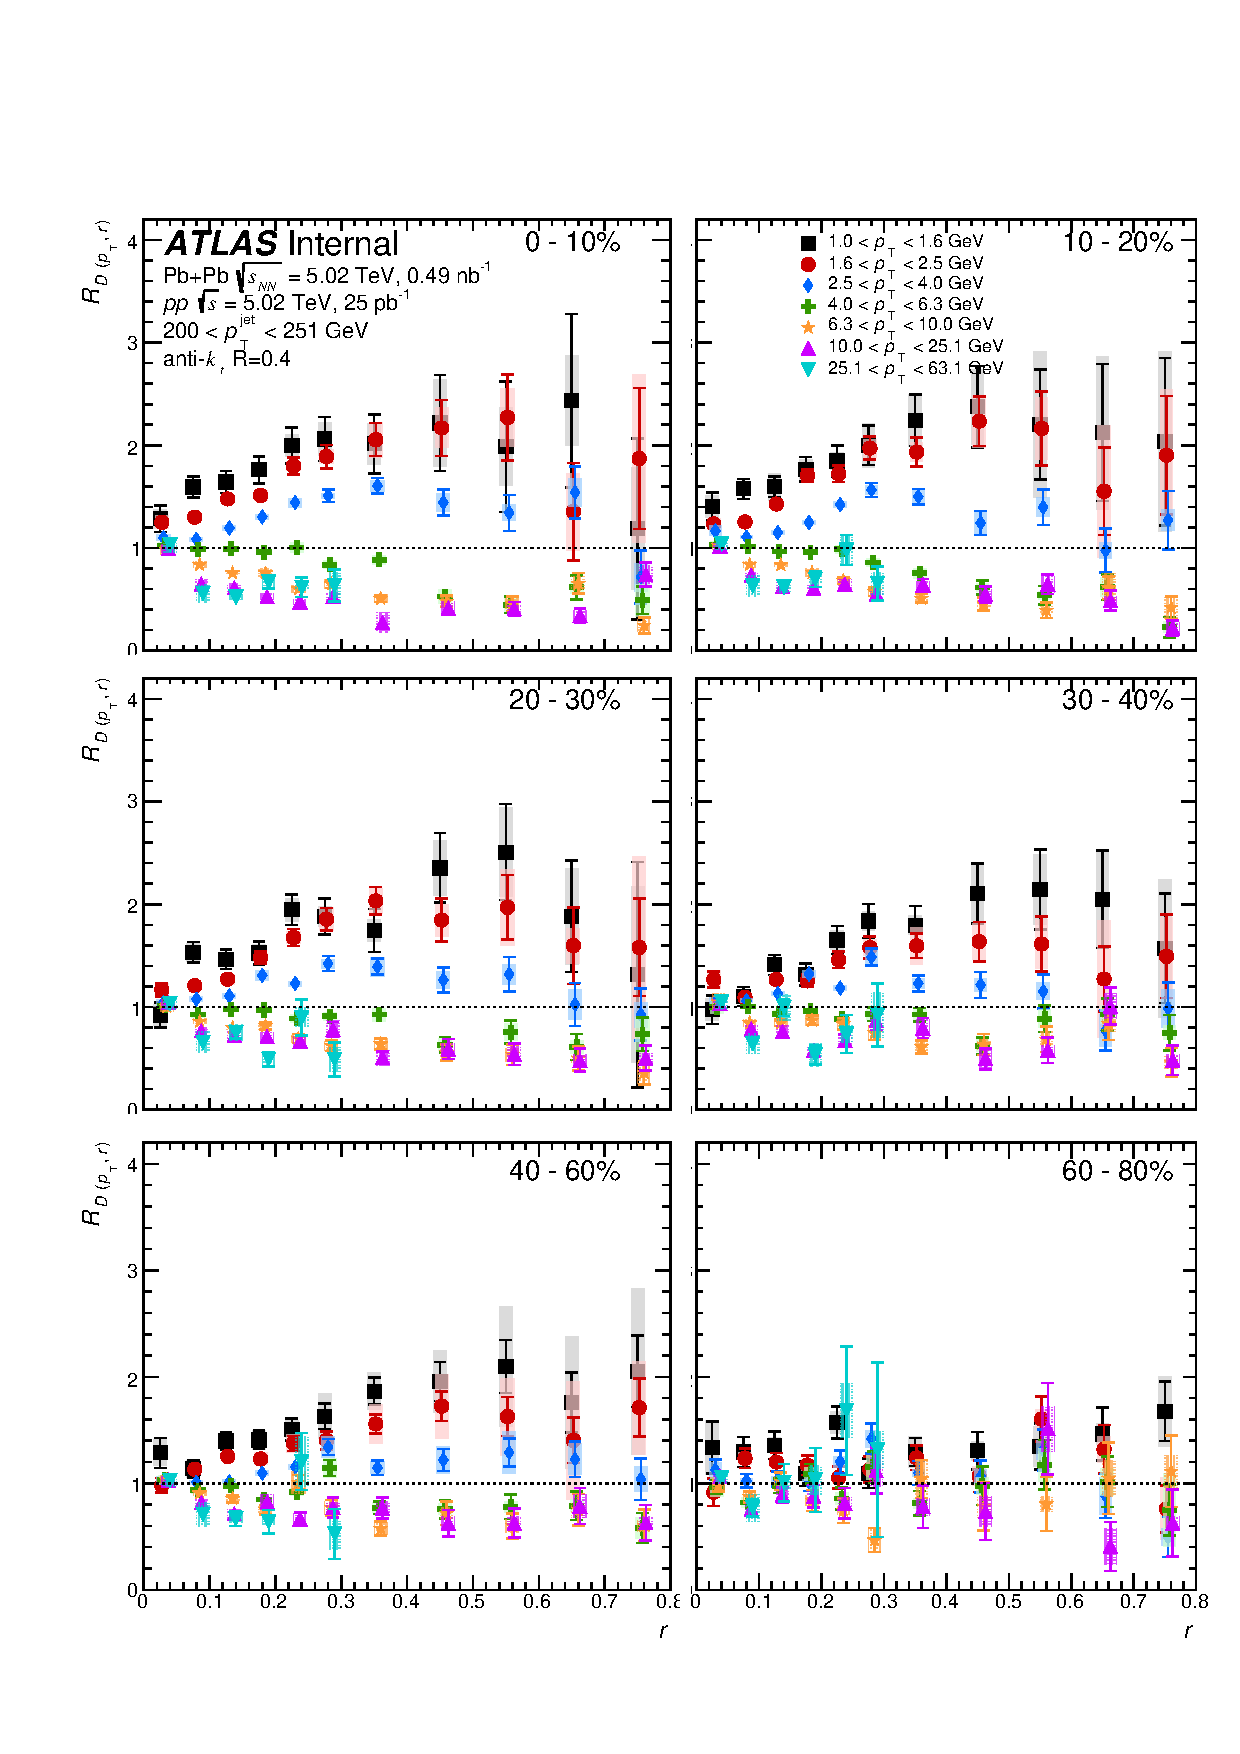
\includegraphics[width=1.0\textwidth]{figures/results/RDpT_dR_jet9}
\caption{The \RDptr\ distributions as a function of \rvar\ for different \pt\ selections in 200--251 GeV jets. The different panels refer to different centrality selections.}
\label{fig:fullset_rptr_j9}
\end{figure}

\begin{figure}[h]
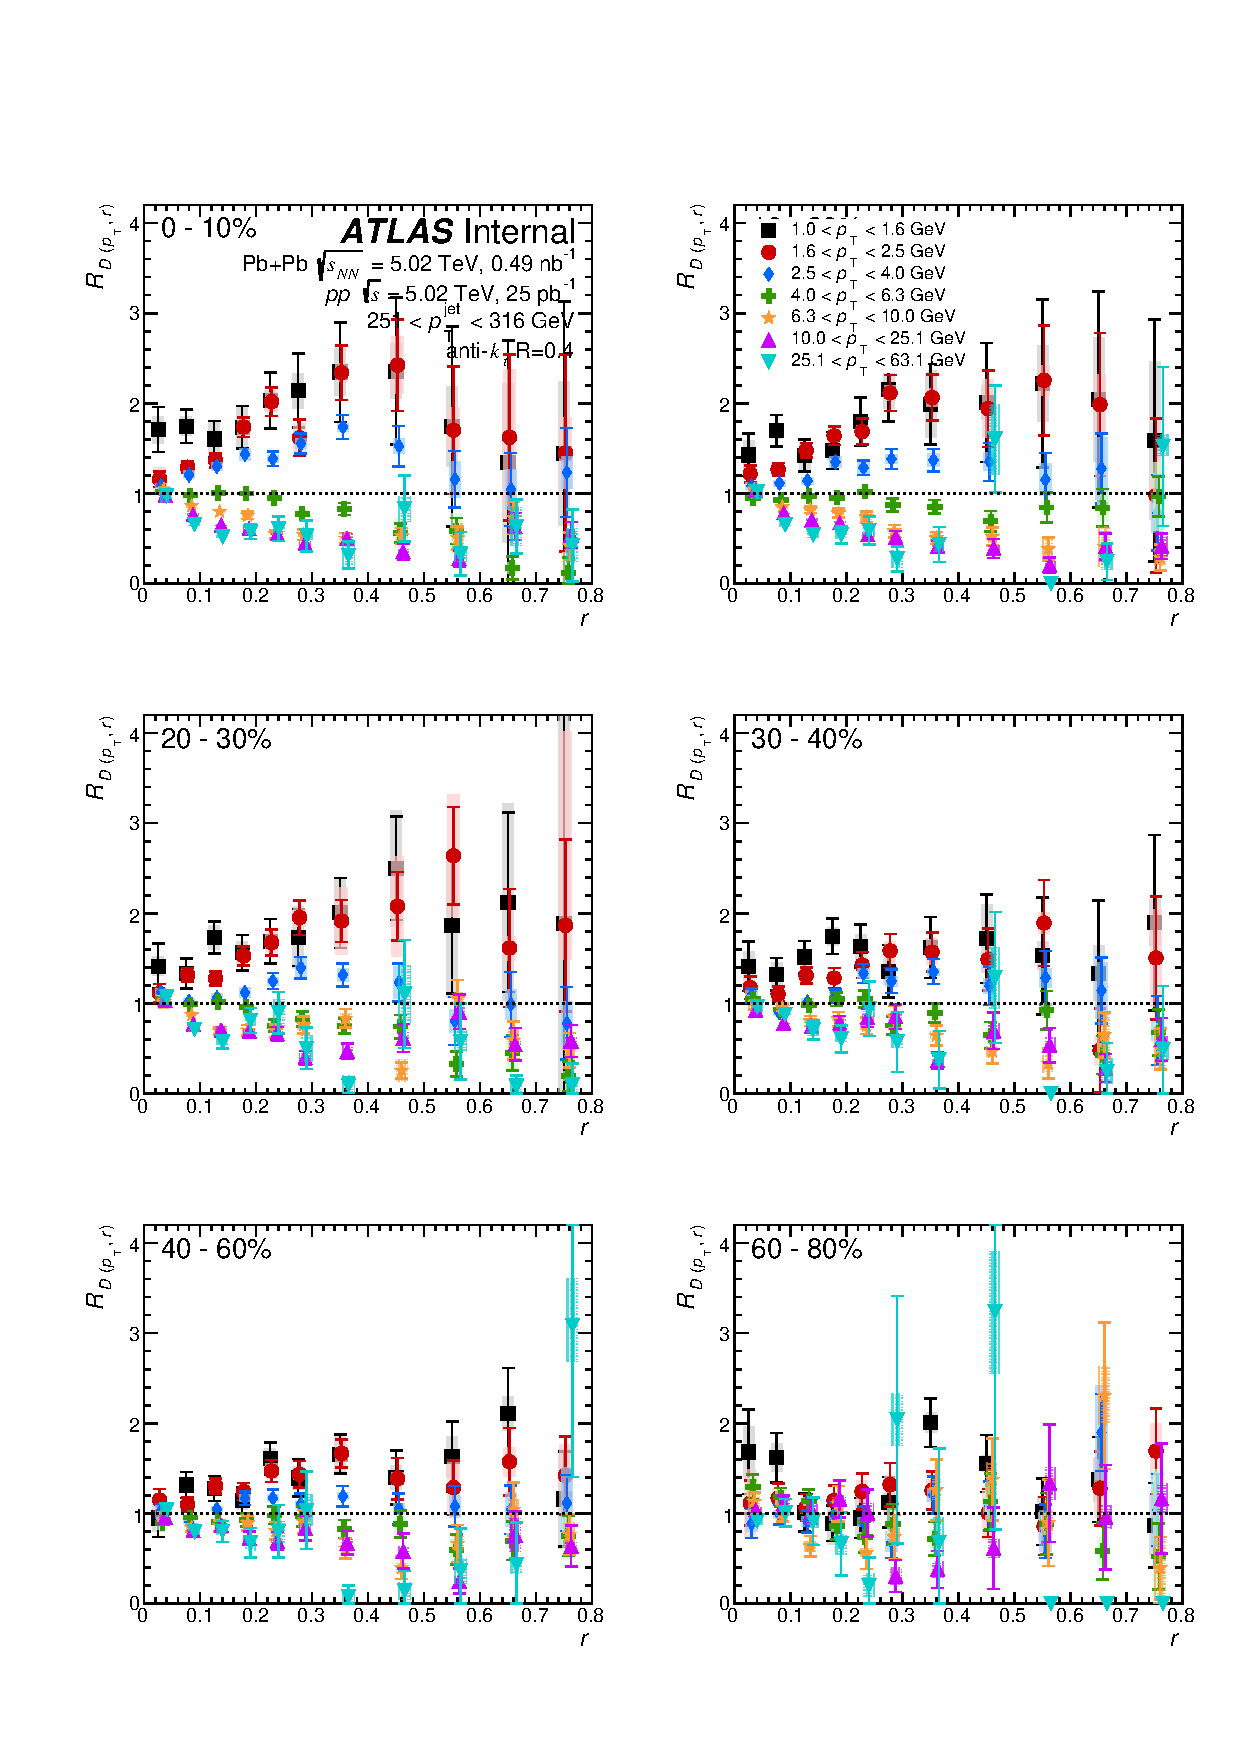
\includegraphics[width=1.0\textwidth]{figures/results/RDpT_dR_jet10}
\caption{The \RDptr\ distributions as a function of \rvar\ for different \pt\ selections in 251--316 GeV jets. The different panels refer to different centrality selections.}
\label{fig:fullset_drtr_j10}
\end{figure}
